% IEEE conference manuscript. Limit: six pages including references.
\documentclass[conference]{IEEEtran}
\IEEEoverridecommandlockouts

\usepackage{cite}
\usepackage{amsmath,amssymb}
\usepackage{booktabs}
\usepackage{graphicx}
\usepackage{textcomp}
\usepackage{xcolor}
\usepackage{url}

\graphicspath{{../../results/RGB/summary/figures/}}
\newcommand{\ph}{\textbf{[PLACEHOLDER]}}

\begin{document}

\title{Lightweight Object Detectors for Real-Time Driver Behavior Detection: A Subject-Disjoint RGB and NIR Benchmark}

\author{
\IEEEauthorblockN{Oumar Mamoun Ibrahim}
\IEEEauthorblockA{\textit{Department of Computer Engineering} \\
\textit{University of Sharjah}, Sharjah, United Arab Emirates \\
U22200741@sharjah.ac.ae}
\and
\IEEEauthorblockN{Mohamad Khairi bin Ishak}
\IEEEauthorblockA{\textit{Department of Computer Engineering} \\
\textit{University of Sharjah}, Sharjah, United Arab Emirates \\
mishak@sharjah.ac.ae}
}

\maketitle

\begin{abstract}
Real-time driver monitoring requires accurate localization of safety-relevant behaviors without excessive latency or nuisance alarms. This paper presents a reproducible benchmark of three unchanged nano-scale object detectors---YOLO11n, YOLO26n, and D-FINE-N---on subject-disjoint visible-light (RGB) and near-infrared (NIR) tracks derived from DMD and Drive\&Act. The protocol retains natural negative frames, separates validation calibration from protected testing, fixes synchronized latency boundaries, and reports three predeclared seeds for RGB. A controlled NIR experiment varies only the training negative-to-positive ratio (2:1 versus 6:1). Across the completed RGB YOLO runs, YOLO11n attains $91.79\pm0.44\%$ $\mathrm{mAP}_{50}$, $86.60\pm0.49\%$ micro-$F_1$, and $68.0\pm1.3$ frames/s, whereas YOLO26n improves $\mathrm{mAP}_{50:95}$ to $56.98\pm0.81\%$ with fewer parameters and estimated FLOPs. Final D-FINE-N and NIR findings are \ph. These controls expose an accuracy--localization--throughput trade-off that conventional frame-randomized comparisons can obscure.
\end{abstract}

\begin{IEEEkeywords}
driver monitoring system, lightweight object detection, subject-disjoint evaluation, near-infrared imaging, false alarms, edge inference
\end{IEEEkeywords}

\section{Introduction}
Driver monitoring systems (DMSs) must recognize visible signs of distraction and fatigue despite changes in identity, illumination, viewpoint, and occlusion. Camera-based methods are non-contact and can localize behavior-specific cues, but deployment quality is not determined by accuracy alone: latency, missed detections, and nuisance alerts all affect usability \cite{michelaraki2023realtime}. This makes evaluation design particularly important for continuously sampled, negative-heavy in-cabin video.

Public datasets support complementary operating conditions. The Driver Monitoring Dataset (DMD) provides multimodal attention and alertness recordings \cite{ortega2020dmd}, while Drive\&Act contains synchronized color, NIR, depth, and pose streams for fine-grained driver activities \cite{martin2019driveact}. Nevertheless, reported results are difficult to compare when neighboring frames or the same driver occur across partitions, background frames are discarded, the test set influences the confidence threshold, or runtime boundaries differ.

Recent work has produced increasingly accurate task-specific lightweight models \cite{wang2024mfyolo,li2024yolosgc,jin2025yolo11cr}. Neutral comparisons of unchanged detector families remain less common, especially across RGB and NIR imagery. This work asks: \emph{under a fixed, leakage-resistant protocol, how do nano-scale convolutional and DETR-family detectors trade localization quality, false alarms, and synchronized inference speed?}

The contributions are threefold:
\begin{itemize}
    \item a subject-disjoint RGB/NIR benchmark that preserves natural negative frames and reports false detections per 100 negative frames alongside COCO AP;
    \item an equal-budget comparison of unchanged YOLO11n, YOLO26n, and D-FINE-N, with three-seed RGB estimates and a controlled NIR training-negative ablation; and
    \item a checksum-backed workflow that separates training, validation-only operating-point selection, and one confirmation-gated protected test pass.
\end{itemize}

\section{Related Work}
\subsection{Lightweight In-Cabin Recognition}
Compact CNN classifiers have demonstrated that parameter count and measured speed must be considered jointly rather than treated as interchangeable \cite{baheti2020mobilevgg}. Hybrid CNN--transformer classification models further target local and global driver-action cues \cite{li2024covit}. For detection, MF-YOLO and YOLO-SGC modify YOLO backbones and feature aggregation for dangerous-driving behaviors \cite{wang2024mfyolo,li2024yolosgc}; YOLO11-CR similarly adds convolution-attention and spatial-calibration modules to a DMD-derived dataset \cite{jin2025yolo11cr}. These studies optimize a proposed architecture. Our aim is instead to compare released nano models without task-specific architectural changes.

\subsection{Controlled Model Comparison}
Comparative studies have evaluated CNNs against vision transformers for distracted-driver recognition \cite{koay2021cnnvit} and multiple YOLO generations for drowsiness detection \cite{herath2025yolocomparison}. The latter uses randomized extracted-frame partitions, so driver and temporal separation are not guaranteed. DETR formulates detection as bipartite set prediction \cite{carion2020detr}; RT-DETR makes this formulation practical for real-time use \cite{zhao2024rtdetr}, and D-FINE refines box-edge distributions for stronger localization \cite{peng2025dfine}.

For NIR driver analysis, PO-GUISE+ uses the front-top Drive\&Act NIR view with driver-disjoint folds and batch-1 FP16 Jetson profiling \cite{pizarro2024poguise}. Driver-disjoint edge prototypes have also emphasized end-to-end latency and stable alerts \cite{ahsani2025edge}. The present benchmark complements those action-recognition systems with frame-level object localization, retained negative frames, validation-only calibration, multi-seed RGB reporting, and identical synchronized profiling boundaries across detector families.

\section{Experimental Protocol}
\subsection{Datasets and Subject-Disjoint Partitions}
Table~\ref{tab:data} summarizes the frozen tracks. The RGB track contains 15,723 face crops sampled at 1 frame/s from 81 DMD recordings of 14 drivers. Each $640\times640$ frame is either a natural negative or contains one of four mutually exclusive cues: \texttt{phone\_use}, \texttt{drinking}, \texttt{yawning}, or \texttt{hand\_over\_mouth}. There are 3,001 positive and 12,722 negative frames. Exhaustive $8{:}3{:}3$ subject assignment minimizes the worst relative cue-distribution deviation, using root-mean-square error as the tie-breaker.

The NIR source pool comprises 3,763 one-second snippets from 30 front-top active-NIR ($850$ nm) Drive\&Act streams and 15 drivers. Ten frames per snippet are sampled at exactly 10 frames/s, cropped to the driver region, and resized to $640\times640$. Human tracklets for \texttt{drinking} and \texttt{phone\_use} are linearly interpolated at 0.1-s intervals. A fixed $9{:}3{:}3$ subject partition is used. Validation and test contain identical ordered examples for every model and ratio.

\begin{table}[t]
\caption{Frozen Subject-Disjoint Dataset Partitions}
\label{tab:data}
\centering
\setlength{\tabcolsep}{3.2pt}
\scriptsize
\begin{tabular}{lccrrrr}
\toprule
Track & Subjects & Rate & Train & Val. & Test & Cues \\
\midrule
RGB & $8/3/3$ & 1 FPS & 9,087 & 3,423 & 3,213 & 4 \\
NIR (1:2) & $9/3/3$ & 10 FPS & 8,100 & 8,810 & 8,500 & 2 \\
NIR (1:6) & $9/3/3$ & 10 FPS & 18,900 & 8,810 & 8,500 & 2 \\
\bottomrule
\end{tabular}
\end{table}

Only the NIR training negatives vary. Both conditions contain 270 positive training snippets; the 1:2 and 1:6 conditions contain 540 and 1,620 negative snippets, respectively. The smaller pool is a subject-stratified, seed-13 subset of the larger pool. NIR is therefore a compact ratio ablation at one seed, not a multi-seed comparison.

\subsection{Models and Training Control}
We use COCO-pretrained YOLO11n and YOLO26n from Ultralytics \cite{ultralytics2026} and D-FINE-N \cite{peng2025dfine}. All runs use $640\times640$ input, physical batch size 8, four-step gradient accumulation (effective batch 32), 220 epochs, automatic mixed precision, and no early stopping. A fixed patch normalizes the final incomplete accumulation window by its actual sample count. Model-native optimization is retained: the Ultralytics \texttt{optimizer=auto} recipe with a linear schedule, and the official D-FINE AdamW/MultiStepLR recipe. RGB uses the predeclared seeds $\{13,37,73\}$ without run selection; all NIR conditions use seed 13.

\subsection{Validation, Protected Test, and Metrics}
The best model-native validation checkpoint is retained. Its confidence threshold is then calibrated only on validation by
\begin{equation}
\tau^*=\underset{\tau\in[0.01,0.99]}{\arg\max}\;F_1(\tau), \qquad
F_1=\frac{2PR}{P+R},
\end{equation}
with higher precision and then higher $\tau$ as tie-breakers. At IoU 0.5, predictions are greedily matched one-to-one within class. We report COCO $\mathrm{mAP}_{50:95}$, $\mathrm{mAP}_{50}$, per-class AP \cite{lin2014coco}, precision $P$, recall $R$, micro-$F_1$, and
\begin{equation}
\mathrm{FAR}_{100}=100\frac{\mathrm{FP}_{\mathrm{neg}}}{N_{\mathrm{neg}}},
\end{equation}
the number of false detections per 100 negative frames. The checkpoint, predictions, data, and selected threshold are checksum-frozen before one explicitly confirmed test pass. RGB values are reported as sample mean $\bar{x}$ and sample standard deviation
\begin{equation}
s=\sqrt{\frac{1}{n-1}\sum_{i=1}^{n}(x_i-\bar{x})^2},\quad n=3.
\end{equation}

Batch-1 FP16 profiling uses an NVIDIA GeForce RTX 4060 8-GB GPU. CUDA synchronization brackets both model-forward and tensor-to-final-detections intervals. Disk I/O, decoding, preprocessing, and metric computation are excluded; p50/p95/p99 latency, sustained FPS, peak allocated VRAM, parameters, and tool-qualified FLOP estimates are recorded.

\section{Results and Discussion}
\subsection{Completed RGB YOLO Benchmark}
Table~\ref{tab:rgbresults} reports the completed six RGB YOLO test runs. YOLO11n obtains the stronger deployment operating point: relative to YOLO26n, it raises micro-$F_1$ by 2.16 percentage points, reduces $\mathrm{FAR}_{100}$ from 0.67 to 0.63, and increases sustained throughput by 31.4\%. YOLO26n instead improves the stricter $\mathrm{mAP}_{50:95}$ by 1.60 points while using slightly fewer parameters and estimated FLOPs. The reversal between $\mathrm{mAP}_{50}$ and $\mathrm{mAP}_{50:95}$ indicates that cue recognition and box tightness should not be conflated.

\begin{table*}[t]
\caption{RGB Subject-Disjoint Test Results: Mean $\pm$ Sample SD over Seeds 13, 37, and 73}
\label{tab:rgbresults}
\centering
\setlength{\tabcolsep}{3.8pt}
\scriptsize
\begin{tabular}{lccccccccc}
\toprule
Model & $\mathrm{mAP}_{50}$ (\%) & $\mathrm{mAP}_{50:95}$ (\%) & $P$ (\%) & $R$ (\%) & $F_1$ (\%) & $\mathrm{FAR}_{100}$ & Lat. (ms) & FPS & M-params/GFLOPs \\
\midrule
YOLO11n & \textbf{91.79$\pm$0.44} & 55.38$\pm$0.41 & \textbf{93.43$\pm$1.16} & \textbf{80.73$\pm$1.70} & \textbf{86.60$\pm$0.49} & \textbf{0.63$\pm$0.04} & \textbf{14.30$\pm$0.20} & \textbf{68.0$\pm$1.3} & 2.59/6.44 \\
YOLO26n & 89.28$\pm$0.99 & \textbf{56.98$\pm$0.81} & 92.56$\pm$1.12 & 77.63$\pm$1.24 & 84.44$\pm$1.14 & 0.67$\pm$0.06 & 19.21$\pm$0.09 & 51.7$\pm$0.2 & \textbf{2.51/5.78} \\
D-FINE-N & \multicolumn{9}{c}{\ph} \\
\bottomrule
\end{tabular}
\end{table*}

The per-class results in Fig.~\ref{fig:rgbplots}(b) clarify the aggregate difference. YOLO11n is stronger for \texttt{yawning} ($0.5998$ versus $0.5613$ AP), whereas YOLO26n is stronger for \texttt{hand\_over\_mouth} ($0.5634$ versus $0.5013$), \texttt{drinking} ($0.6174$ versus $0.6072$), and \texttt{phone\_use} ($0.5371$ versus $0.5069$). The largest seed variability occurs for the two visually subtle mouth-related cues, supporting multi-seed rather than single-run RGB reporting.

\begin{figure*}[t]
\centering
\begin{minipage}[t]{0.48\textwidth}
    \centering
    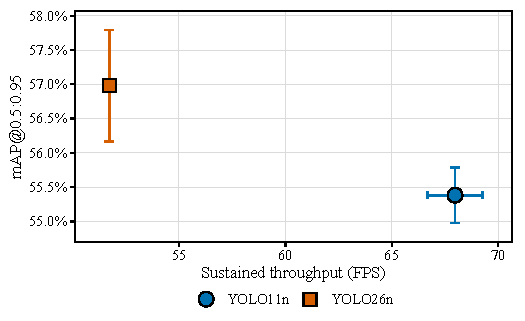
\includegraphics[width=\linewidth]{accuracy_vs_speed.pdf}
    \vspace{-1.5ex}\centerline{\scriptsize(a) Accuracy--throughput trade-off.}
\end{minipage}\hfill
\begin{minipage}[t]{0.48\textwidth}
    \centering
    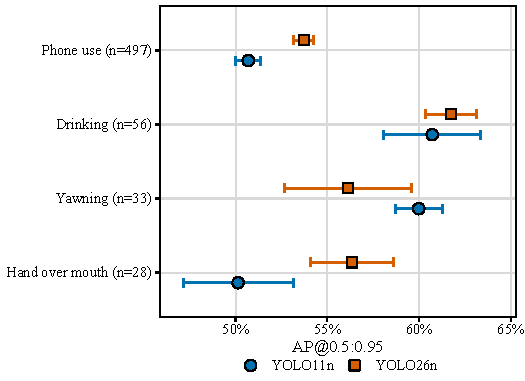
\includegraphics[width=\linewidth]{per_class_ap.pdf}
    \vspace{-1.5ex}\centerline{\scriptsize(b) Per-class $\mathrm{AP}_{50:95}$.}
\end{minipage}
\caption{Completed RGB YOLO benchmark. Error bars denote sample SD across seeds 13, 37, and 73. In (a), marker area is proportional to the serialized inference artifact size. Both plots were generated from the frozen aggregate using R/ggplot2.}
\label{fig:rgbplots}
\end{figure*}

\subsection{Pending D-FINE-N and NIR Results}
The declared completion matrix is shown in Table~\ref{tab:nirresults}. No interim checkpoint or partial test value is substituted. After all frozen runs complete, this section will report: (i) the best overall RGB detector under strict AP and deployment operating-point criteria; (ii) whether D-FINE-N changes the CNN--DETR trade-off; and (iii) the effect of added NIR training negatives with validation/test held identical. The resulting comparison is \ph.

\begin{table}[t]
\caption{NIR Test Results at Seed 13}
\label{tab:nirresults}
\centering
\setlength{\tabcolsep}{3pt}
\scriptsize
\begin{tabular}{llccccc}
\toprule
Model & Ratio & $\mathrm{mAP}_{50:95}$ & $F_1$ & $\mathrm{FAR}_{100}$ & Lat. & FPS \\
\midrule
YOLO11n & 1:2 & \multicolumn{5}{c}{\ph} \\
YOLO11n & 1:6 & \multicolumn{5}{c}{\ph} \\
YOLO26n & 1:2 & \multicolumn{5}{c}{\ph} \\
YOLO26n & 1:6 & \multicolumn{5}{c}{\ph} \\
D-FINE-N & 1:2 & \multicolumn{5}{c}{\ph} \\
D-FINE-N & 1:6 & \multicolumn{5}{c}{\ph} \\
\bottomrule
\end{tabular}
\end{table}

\subsection{Limitations}
RGB and NIR use different datasets and ontologies; their results are separate operating tracks, not a paired spectral domain-shift experiment. Subject-disjoint splits reduce identity leakage but do not establish generalization to unseen cameras, cabins, countries, or clinical fatigue states. NIR uses one seed, so the ratio ablation does not estimate stochastic variance. Interpolated NIR boxes can miss rapid nonlinear motion, and the single-cue ontology excludes concurrent behaviors. Finally, RTX 4060 latency is hardware-specific and must be re-profiled on the intended edge target. These constraints bound the claims to visible cue localization under the stated protocol.

\section{Conclusion}
The completed RGB YOLO benchmark shows that the preferred nano detector depends on the deployment objective: YOLO11n provides higher throughput, micro-$F_1$, and $\mathrm{mAP}_{50}$, whereas YOLO26n provides tighter localization by $\mathrm{mAP}_{50:95}$ with marginally fewer parameters and FLOPs. Subject-disjoint partitions, retained negatives, validation-only calibration, multi-seed estimates, and synchronized runtime boundaries make that conclusion more defensible than AP or nominal model size alone. The final three-model RGB ranking, NIR negative-ratio effect, and cross-track conclusion are \ph.

\section*{Data and Code Availability}
Authored annotations, subject partitions, checksums, evaluation code, and result artifacts are available in the project repository. DMD and Drive\&Act media remain subject to their original licenses; users with access can reconstruct both tracks using the published scripts. Checkpoints remain local.

\IEEEtriggeratref{11}
\bibliographystyle{IEEEtran}
\bibliography{references}

\end{document}
